\documentclass[11pt,svgnames,smaller]{beamer}

\usepackage{CommandsAndStyle}

\usepackage{listings}
\usepackage{amsthm}
\usepackage{amsmath}
\usepackage{subfig}
\usepackage{xcolor}
\usepackage{textpos}
\usepackage{transparent}
\usepackage{tikz}
\usepackage{epigraph}
\usepackage[ruled,vlined,linesnumbered]{algorithm2e}
\usepackage{amsmath,amsfonts,amssymb,amsthm}
\usepackage{latexsym}
\usepackage{graphicx} 
\usepackage{wrapfig}
\usepackage{array, makecell} %
\usepackage{hyperref}
\usepackage{caption}

\captionsetup[figure]{labelformat=empty}% redefines the caption setup of the figures environment in the beamer class.

\mode<presentation>

\author{Gaspare Ferraro}

\author[Gaspare Ferraro]{
\includegraphics[height=2cm]{images/cherubino}\\Gaspare Ferraro\\ \vspace{10pt} \small{ICT Risk Assessment}}
\institute[University Pisa]{University of Pisa\\Master Degree in Computer Science}

\setbeamertemplate{section page}
{
	\begin{centering}
		\begin{beamercolorbox}[sep=16pt,center]{part title}
			\usebeamerfont{section title}\insertsection\par
		\end{beamercolorbox}
	\end{centering}
}

\title{The Dark Side of the ForSSHe}
\subtitle{A landscape of OpenSSH backdoors}
\date{Pisa, \today}
\titlegraphic{\vfill}

\setbeamercolor{title}{fg=black!65!black}

\begin{document}
	
	\begin{frame} 
	\titlepage
	\end{frame}
				
	\logo{\transparent{0.2}
\includegraphics[height=2cm]{images/cherubino}}

	\part{Introduction}
\section{Introduction}

\begin{frame}
	\partpage
\end{frame}

\begin{frame}
	\frametitle{SSH}
\end{frame}

\begin{frame}
	\frametitle{OpenSSH suite}
\end{frame}

\begin{frame}
	\frametitle{The attackers}
\end{frame}

\begin{frame}
	\frametitle{Operation Windigo}
\end{frame}

	\part{Chapter 2}

\begin{frame}
	\partpage
\end{frame}

\begin{frame}
	\frametitle{Slides 4}
\end{frame}

\begin{frame}
	\frametitle{Slides 5}
\end{frame}

\begin{frame}
	\frametitle{Slides 6}
\end{frame}

	\part{Chapter 3}

\begin{frame}
	\partpage
\end{frame}

\begin{frame}
	\frametitle{Slides 7}
\end{frame}

\begin{frame}
	\frametitle{Slides 8}
\end{frame}

\begin{frame}
	\frametitle{Slides 9}
\end{frame}

	\part{Honeypot}
\section{Honeypot}

\begin{frame}
	\partpage
\end{frame}

%%%%%%%%%%%%%%%%%%%%%%%%%%%%%%%%%%%%%%%%%%%%%%%%%%%%%%%%%%%%%%%%%%%%%%%%%%%%%%%
\begin{frame}
	\frametitle{Definition and goals}
	
	A honeypot is a ICT resource used for monitoring, detecting and analyzing attacks. It has no production value, no real sensible data. 
	
	\smallskip

	Can be classified by its implementation (virtual or physical), purpose (prevention, detection, research) and level of interaction (low, middle, high) in particular:
	
	\medskip

	\textbf{Low-interaction honeypots} simulate only some aspects of the system, while limiting the ability of the attacker. More easy to deploy but can get a limited amount of information.
	
	\medskip
	
	\textbf{High-interaction honeypots} based on a real OS, the attackers gets full access to the system and can be compromised completely (with an higher risk). Harder to deply and manage but can get a full overview of the attackers.
	
	\medskip

  Many OpenSSH honeypot solutions exists but due to their popularity they are easy to detect.
  
	\smallskip

  An high-interaction custom honeypot was chosen in order to maximize the information gathered from the attackers.
  	
\end{frame}
%%%%%%%%%%%%%%%%%%%%%%%%%%%%%%%%%%%%%%%%%%%%%%%%%%%%%%%%%%%%%%%%%%%%%%%%%%%%%%%


%%%%%%%%%%%%%%%%%%%%%%%%%%%%%%%%%%%%%%%%%%%%%%%%%%%%%%%%%%%%%%%%%%%%%%%%%%%%%%%
\begin{frame}
	\frametitle{Honeypot structure and strategy}
	
	\footnotesize
	
  Credentials are leaked in two different ways.
  
  \smallskip

  For a client backdoor is enough to log into the honeypot server. 
  
  \smallskip

  More complicate is for a daemon backdoor, one solution is to install the daemon backdoor on the honeypot server, 
  log in with a safe client and remove the backdoor, in order to simulate the backdoor detection in the attacker eyes.

  \smallskip

  \begin{center}    
  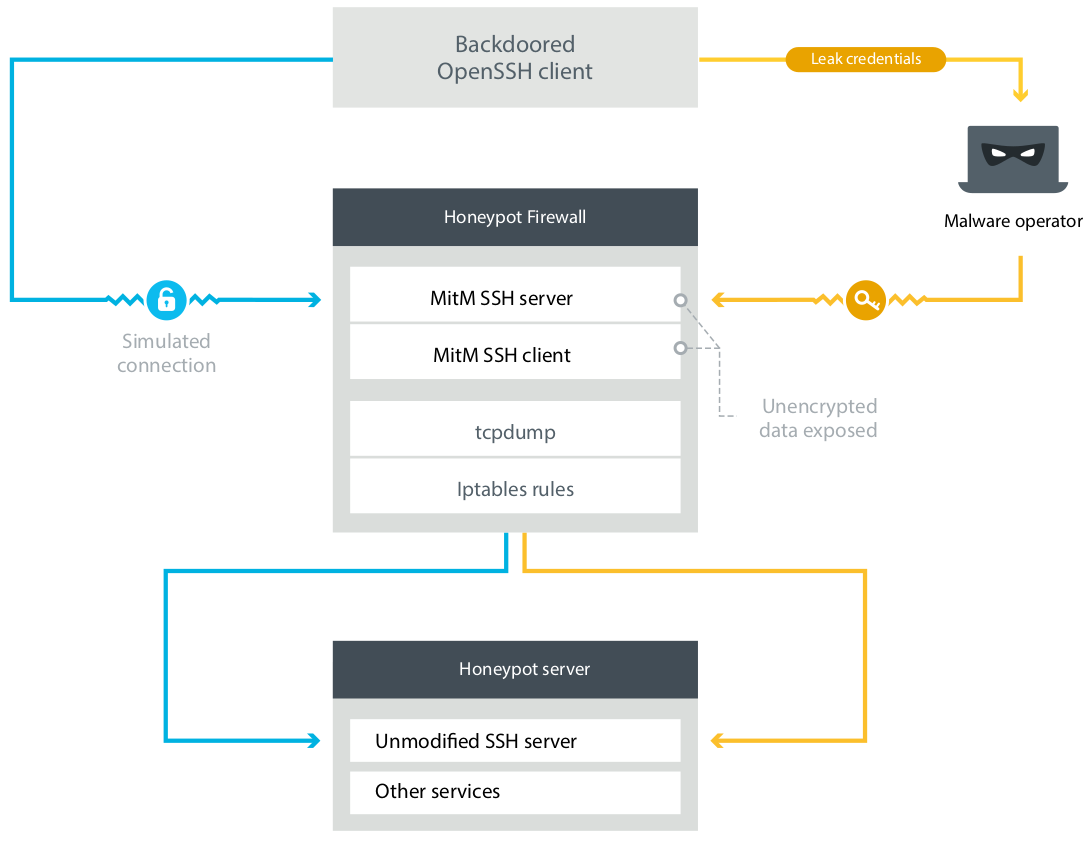
\includegraphics[width=0.5\textwidth]{images/honeypot_infrastructure}
  \captionof{figure}{Honeypot infrastructure}
  \end{center}

\end{frame}
%%%%%%%%%%%%%%%%%%%%%%%%%%%%%%%%%%%%%%%%%%%%%%%%%%%%%%%%%%%%%%%%%%%%%%%%%%%%%%%


%%%%%%%%%%%%%%%%%%%%%%%%%%%%%%%%%%%%%%%%%%%%%%%%%%%%%%%%%%%%%%%%%%%%%%%%%%%%%%%
\begin{frame}
	\frametitle{Observed interaction: Minban}
	
	Both client and server backdoors were available, of course the backdoor client was used to leak the credentials.
	
	\smallskip
	
	The attackers behing the backdoor logged in to the honeypot after few hours of leaking and thanks to the architecture the commands executed on the server were logged.
	
	\smallskip
	
  \begin{center}    
  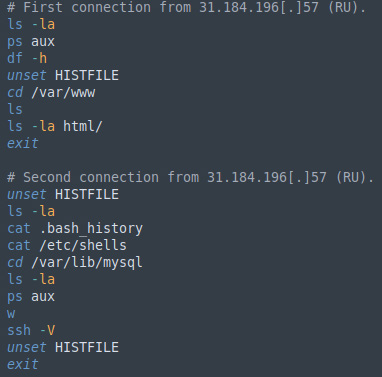
\includegraphics[width=0.25\textwidth]{images/minban}
  \captionof{figure}{Attackers command captured for Minban}
  \end{center}
  
	\smallskip
	
  Attackers logged in manually from a Russian IP address, try to clean command history, check some files and finally check the version of OpenSSH binary.  

\end{frame}
%%%%%%%%%%%%%%%%%%%%%%%%%%%%%%%%%%%%%%%%%%%%%%%%%%%%%%%%%%%%%%%%%%%%%%%%%%%%%%%


%%%%%%%%%%%%%%%%%%%%%%%%%%%%%%%%%%%%%%%%%%%%%%%%%%%%%%%%%%%%%%%%%%%%%%%%%%%%%%%
\begin{frame}
	\frametitle{Observed interaction: Borleias}
	
	More interesting the results of the Borleias backdoor: the attackers first logged into the honeypot in less than 24 hours and repeat for more than 10 times withing four days.
	
	\smallskip
	
	\begin{itemize}
	  \item The attackers used Tor to login, in order to not leave trace.
	  \item A classic version of the OpenSSH client was used to connect.
	  \item They managed to get the credential leaked in the Mimban operations: this means that there is a connection between the two backdoors (maybe same operators or the credentials were sold somewhere).
	  \item Some basic checks at beginning then more interesting operations in the few days later, in particular they drop a new version of the backdoor.
	  \item Gather all the information about the server, exfiltrate them and clean all the command history.
	  \item Meticulous attention to details (check of running process, timestamps of files, logged-in users between the execution of each command, ...)
	\end{itemize} 
	
\end{frame}
%%%%%%%%%%%%%%%%%%%%%%%%%%%%%%%%%%%%%%%%%%%%%%%%%%%%%%%%%%%%%%%%%%%%%%%%%%%%%%%

	\part{Mitigation}
\section{Mitigation}

\begin{frame}
	\partpage
\end{frame}

%%%%%%%%%%%%%%%%%%%%%%%%%%%%%%%%%%%%%%%%%%%%%%%%%%%%%%%%%%%%%%%%%%%%%%%%%%%%%%%
\begin{frame}
	\frametitle{Preventing compromise of SSH servers}
	
	
	Very difficult to determine the infection vector used to install these OpenSSH backdoors.
	
	\medskip
	
	In the operation Windigo two different vector was used: 
	
	\smallskip
	
	An attack of the website \textit{kernel.org} (the official repository of the linux kernel source code) to inject malicious code.
	
	\smallskip
	
	An attack to \textit{cpanel.net}, the most famous software to manage websites and hosting.

  \medskip
  
  Obvious but important recommendation is to install software only from trusted sources, e.g. checks sources in \textsc{/etc/apt/sources.list} for debian-derived linux distribution or install only trusted package from the AUR (Arch User Repository) for ArchLinux distribution. 
  	
\end{frame}
%%%%%%%%%%%%%%%%%%%%%%%%%%%%%%%%%%%%%%%%%%%%%%%%%%%%%%%%%%%%%%%%%%%%%%%%%%%%%%%


%%%%%%%%%%%%%%%%%%%%%%%%%%%%%%%%%%%%%%%%%%%%%%%%%%%%%%%%%%%%%%%%%%%%%%%%%%%%%%%
\begin{frame}
	\frametitle{Correct OpenSSH configuration}
\end{frame}
%%%%%%%%%%%%%%%%%%%%%%%%%%%%%%%%%%%%%%%%%%%%%%%%%%%%%%%%%%%%%%%%%%%%%%%%%%%%%%%


%%%%%%%%%%%%%%%%%%%%%%%%%%%%%%%%%%%%%%%%%%%%%%%%%%%%%%%%%%%%%%%%%%%%%%%%%%%%%%%
\begin{frame}
	\frametitle{Check logs}
	
	Enable logs for every critical service.

	\smallskip

  Periodically backup logs in an external server/device.

	\smallskip
	
	Check for log files in server.

	\smallskip
	
  \begin{center}    
  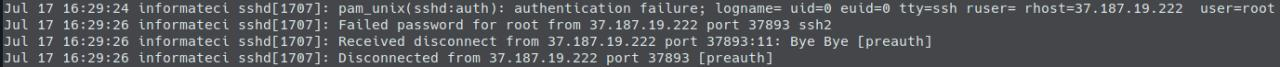
\includegraphics[width=1\textwidth]{images/ssh_log}
  \captionof{figure}{Failed attempt of login in a server}
  \end{center}

\end{frame}
%%%%%%%%%%%%%%%%%%%%%%%%%%%%%%%%%%%%%%%%%%%%%%%%%%%%%%%%%%%%%%%%%%%%%%%%%%%%%%%

%%%%%%%%%%%%%%%%%%%%%%%%%%%%%%%%%%%%%%%%%%%%%%%%%%%%%%%%%%%%%%%%%%%%%%%%%%%%%%%
\begin{frame}
	\frametitle{Analyze network traffic}
\end{frame}
%%%%%%%%%%%%%%%%%%%%%%%%%%%%%%%%%%%%%%%%%%%%%%%%%%%%%%%%%%%%%%%%%%%%%%%%%%%%%%%

%%%%%%%%%%%%%%%%%%%%%%%%%%%%%%%%%%%%%%%%%%%%%%%%%%%%%%%%%%%%%%%%%%%%%%%%%%%%%%%
\begin{frame}
	\frametitle{Detect compromised SSH tools}
\end{frame}
%%%%%%%%%%%%%%%%%%%%%%%%%%%%%%%%%%%%%%%%%%%%%%%%%%%%%%%%%%%%%%%%%%%%%%%%%%%%%%%

	
	\section{Conclusion}
	\begin{frame}
		\frametitle{Conclusion}
		\centering
		
		\begin{itemize}
		  \item A compromised server can compromise other servers and milions of users (see Carbanak operation).
		  \item Install software only from trusted origin.
		  \item Keep system up-to-date (upgrade always to the last \textit{stable} version).
		  \item Correct configure software.
		  \item Prefer public/private key login instead of password login.
		  \item Setup a multi factor authentication.
		  \item Check logs periodically for strange activities.
		  \item Keep track of external connections and setup correctly a firewall.
		\end{itemize}
 	\end{frame}
  
	\section{References}
	\begin{frame}
		\frametitle{References}
		
		\footnotesize
		
    \textbf{[1] The Dark Side of the ForSSHe, ESET}\\
    \url{https://www.welivesecurity.com/wp-content/uploads/2018/12/ESET-The_Dark_Side_of_the_ForSSHe.pdf}

    \smallskip

    \textbf{[2] The Dark Side of the ForSSHe, ESET}\\
    \url{https://www.welivesecurity.com/2018/12/05/dark-side-of-the-forsshe/}

    \smallskip

    \textbf{[3] Linux/SSHDoor.A Backdoored SSH daemon that steals passwords, ESET}\\
    \url{https://www.welivesecurity.com/2013/01/24/linux-sshdoor-a-backdoored-ssh-daemon-that-steals-passwords/}

    \smallskip

    \textbf{[4] Operation Windigo, ESET}\\
    \url{https://www.welivesecurity.com/wp-content/uploads/2014/03/operation_windigo.pdf}

    \smallskip

    \textbf{[5] ESET discovers 12 previously undetected Linux backdoors, ESET}\\
    \url{https://www.eset.com/int/about/newsroom/press-releases/research/eset-discovers-12-previously-undetected-linux-backdoors/}

    \smallskip

    \textbf{[6] Openssh backdoor used on compromised Linux servers, randhome}\\
    \url{https://www.randhome.io/blog/2016/08/01/openssh-backdoor-used-on-compromised-linux-servers/}

    \smallskip

    \textbf{[7] Carbanak APT: The great bank robbery, Kaspersky}\\
    \url{https://media.kasperskycontenthub.com/wp-content/uploads/sites/43/2018/03/08064518/Carbanak_APT_eng.pdf}


 	\end{frame}
  
\end{document}
